\section{Konzeptidee / Lösungsansatz}

Das vorgestellte Grobkonzept verfolgt das Ziel, den aktuell manuellen Verpackungsprozess der Bremssysteme vollständig zu automatisieren. Die zentrale Idee besteht darin, eine automatisierte Verpackungsanlage zu integrieren, die über ein Roboterhandling, eine angepasste Fördertechnik und eine modulare Steuerungseinheit verfügt. Die Anlage soll in die bestehende Produktionslinie eingebunden werden, ohne den laufenden Produktionsfluss wesentlich zu beeinträchtigen.\\

Die Verpackungsanlage besteht aus mehreren Hauptkomponenten:
\begin{itemize}
	\item \textbf{Industrieroboter:} Übernimmt das automatische Greifen, Positionieren und Ablegen der Bremssysteme in die Verpackungen. Der Roboter wird über eine SPS gesteuert und erhält über Profibus bzw. Profinet die Prozesssignale\cite{ABB_Applications}.
	\item \textbf{Fördertechnik:} Dient der Zuführung der fertigen Produkte und der Abführung der verpackten Einheiten. Diese ist mit Sensorik zur Teileerkennung und Stauüberwachung ausgestattet.
	\item \textbf{Verpackungsstation:} Beinhaltet die Vorrichtungen zum Einlegen, Zufalten und Verschließen der Verpackung. Dieser Schritt kann mechanisch oder pneumatisch ausgeführt werden.
	\item \textbf{Steuerung und Kommunikation:} Eine zentrale SPS (z. B. Siemens S7 oder Beckhoff) übernimmt die Ablaufsteuerung und kommuniziert mit der Robotersteuerung, der Fördertechnik sowie der übergeordneten Produktionsleittechnik.
\end{itemize}

Das Anlagenlayout ist modular aufgebaut, sodass spätere Anpassungen oder Erweiterungen möglich sind. Die Einbindung erfolgt am Ende der bestehenden Produktionslinie, wo die manuelle Verpackungsstation bisher betrieben wird. Dadurch kann die Anlage schrittweise integriert und getestet werden, ohne den Serienbetrieb vollständig zu unterbrechen.\\

\subsection{Ablauf des Verpackungsprozesses}

Der geplante Ablauf der automatisierten Verpackung lässt sich wie folgt beschreiben:
\begin{enumerate}
	\item Das fertige Bremssystem wird vom Förderband der Montageanlage auf die Verpackungseinheit übergeben.
	\item Ein Industrieroboter greift das Produkt mithilfe eines speziell angepassten Greifers.
	\item Der Roboter positioniert das Produkt präzise in der Verpackung und überprüft die Lage mittels Sensorik oder Kamerasystem.
	\item Nach erfolgreichem Einlegen wird die Verpackung automatisch verschlossen.
	\item Die fertige Verpackung wird über das Abführband abtransportiert und einem Palettier- oder Versandbereich übergeben.
\end{enumerate}
Der dargestellte Ablauf zeigt, dass die automatisierte Verpackung eine klar strukturierte 
und reproduzierbare Prozesskette bildet. Durch die Kombination aus robotergestützter Handhabung, 
sensorbasierter Lagekontrolle und automatischem Verpackungsabschluss entsteht ein stabiler und 
effizienter Prozess, der unabhängig von manuellen Einflüssen eine gleichbleibend hohe Qualität 
gewährleistet. Das folgende Ablaufdiagramm visualisiert den Prozess und stellt die einzelnen 
Schritte sowie deren logische Abfolge übersichtlich dar.

Zur Veranschaulichung des Prozesses dient das nachfolgende Ablaufdiagramm.

\begin{figure}[H]
	\centering
	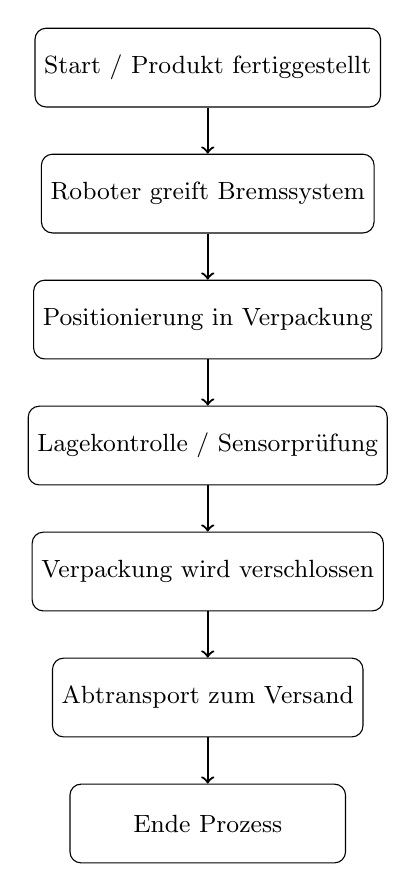
\begin{tikzpicture}[
		node distance=1.6cm,
		every node/.style={rectangle, rounded corners, draw=black, align=center, minimum width=3.5cm, minimum height=1cm, font=\small}
		]
		\node (start) {Start / Produkt fertiggestellt};
		\node (rob) [below of=start] {Roboter greift Bremssystem};
		\node (pos) [below of=rob] {Positionierung in Verpackung};
		\node (check) [below of=pos] {Lagekontrolle / Sensorprüfung};
		\node (seal) [below of=check] {Verpackung wird verschlossen};
		\node (out) [below of=seal] {Abtransport zum Versand};
		\node (end) [below of=out] {Ende Prozess};
		
		\draw[->, thick] (start) -- (rob);
		\draw[->, thick] (rob) -- (pos);
		\draw[->, thick] (pos) -- (check);
		\draw[->, thick] (check) -- (seal);
		\draw[->, thick] (seal) -- (out);
		\draw[->, thick] (out) -- (end);
	\end{tikzpicture}
	\caption{Ablaufdiagramm des automatisierten Verpackungsprozesses}
	\label{fig:prozessablauf}
\end{figure}

\subsection{Signalfluss und Kommunikation}

Die Kommunikation zwischen den Anlagenkomponenten erfolgt über ein industrielles Bussystem. Der Roboter erhält Steuerbefehle und Statusmeldungen über digitale Ein- und Ausgänge der SPS. Die Fördertechnik liefert Rückmeldungen über Positions- und Stausensoren. Ein schematischer Signalfluss ist in Abbildung \ref{fig:signalfluss} dargestellt.\\
Neben den dargestellten Hauptsignalen werden im praktischen Anlagenbetrieb zahlreiche weitere 
Informations- und Diagnosesignale übertragen, die für einen störungsfreien Ablauf notwendig 
sind. Dazu gehören unter anderem Statusmeldungen der Sicherheitsmodule, Diagnosedaten der 
Feldgeräte sowie interne Systeminformationen der Steuerung. Durch die einheitliche 
Kommunikationsstruktur lassen sich diese Daten zentral auswerten, was die Instandhaltung 
erheblich erleichtert und eine schnellere Reaktion auf Prozessabweichungen ermöglicht. 
Darüber hinaus bildet der strukturierte Signalfluss die Grundlage für zukünftige Erweiterungen 
der Anlage, etwa die Integration zusätzlicher Sensorik oder weiterer automatisierter 
Prozessschritte.

\begin{figure}[H]
	\centering
	\begin{tikzpicture}[
		font=\small,
		node distance=1.4cm and 4.2cm,
		box/.style={
			draw,
			rounded corners,
			minimum width=4.0cm,
			minimum height=1.0cm,
			align=center,
			fill=gray!10
		},
		spsbox/.style={
			draw,
			rounded corners,
			minimum width=4.5cm,
			minimum height=6.5cm,
			align=center,
			font=\small\bfseries,
			fill=blue!10
		},
		arrow/.style={
			thick,
			-{Latex[length=3mm]},
		}
		]
		
		% --- SPS links ---
		\node[spsbox] (sps) {Beckhoff SPS\\(TwinCAT 3 / EtherCAT Master)};
		
		% --- Geräte rechts, exakt untereinander ---
		\node[box, fill=orange!15, right=of sps, yshift=2.5cm] (robot) {ABB Industrieroboter}; % auf Höhe Profinet
		\node[box, fill=green!15, right =of sps, yshift=1.25cm] (belt) {Fördertechnik / Aktoren}; % auf Höhe EtherCAT
		\node[box, fill=yellow!15, right=of sps, yshift=0cm] (sensor) {Sensorik / Lichtschranken}; % auf Höhe EtherCAT
		\node[box, fill=cyan!20, right=of sps, yshift=-1.25cm] (hmi) {Windows-PC / HMI-Client}; % auf Höhe Ethernet
		\node[box, fill=gray!20, right=of sps, yshift=-2.5cm] (mes) {MES / Leitsystem}; % auf Höhe OPC UA
		
		
		% --- Pfeile (kurz & waagrecht, mit Beschriftung) ---
		\draw[arrow] (sps.east)++(0,2.5) -- ++(2,0) node[midway, above]{\textbf{Profinet}} |- (robot.west);
		\draw[arrow] (sps.east)++(0,1.25) -- ++(2,0) node[midway, above]{\textbf{EtherCAT}} |- (belt.west);
		\draw[arrow] (sps.east)++(0,0) -- ++(2,0) node[midway, above]{\textbf{EtherCAT}} |- (sensor.west);
		\draw[arrow, dashed] (sps.east)++(0,-1.25) -- ++(3.5,0) node[midway, above]{\textbf{Ethernet / TCP-IP}} |- (hmi.west);
		\draw[arrow, dashed] (sps.east)++(0,-2.5) -- ++(3,0) node[midway, above]{\textbf{OPC UA / TCP}} |- (mes.west);
		
		% --- Legende ---
		\node[draw, fill=white, below=1.4cm of mes, align=left, font=\footnotesize, inner sep=3pt] (legende) {
			\textbf{Legende:}\\[2pt]
			\tikz{\draw[arrow] (0,0) -- ++(0.7,0);} \quad Echtzeit-Feldbus (Profinet / EtherCAT)\\[3pt]
			\tikz{\draw[arrow, dashed] (0,0) -- ++(0.7,0);} \quad IT-Kommunikation / Visualisierung
		};
		
	\end{tikzpicture}
	\caption{Kommunikationsstruktur der automatisierten Verpackungsanlage mit parallelen Signalverbindungen}
	\label{fig:signalfluss}
\end{figure}

In der Grafik \ref{fig:signalfluss} sind die verschiedenen Schnittstellen und Kommunikationspfade der Anlage dargestellt. Die \textbf{SPS} bildet dabei das zentrale Element der Steuerungsarchitektur\cite{Anwendung_IEC61131}\cite{OPC_IEC61131}. Durch den Einsatz einer Beckhoff-Steuerung ist es möglich, einheitlich über das Hauptbussystem \textbf{EtherCAT} über alle Feldebenen\cite{Automatisierungspyramide} hinweg zu kommunizieren. Dies vereinfacht nicht nur die Inbetriebnahme, sondern reduziert auch den Schulungsaufwand für das Fachpersonal.\\

Da alle Beckhoff-Komponenten nativ über EtherCAT angebunden werden können, entsteht eine durchgängige, echtzeitfähige Kommunikationsstruktur. Dadurch können Sensoren, Aktoren und Förderkomponenten effizient integriert und synchronisiert werden \cite{Beckhoff}.\\

Der in der Anlage verwendete \textbf{ABB-Industrieroboter} unterstützt hingegen keine EtherCAT-Schnittstelle, weshalb die Kommunikation hier über \textbf{Profinet} realisiert wird. Die Verbindung zwischen Robotersteuerung und SPS erfolgt über definierte Signale, wodurch eine sichere und deterministische Prozessabfolge gewährleistet ist.\\

Durch diese Kombination aus EtherCAT und Profinet entsteht ein hybrides, aber flexibles Kommunikationskonzept, das eine hohe Kompatibilität zwischen unterschiedlichen Herstellern ermöglicht. Dies gewährleistet sowohl die funktionale Erweiterbarkeit der Anlage als auch eine langfristige Zukunftssicherheit des Steuerungskonzepts.\\

Über die Ethernet-Schnittstelle beziehungsweise das \textbf{OPC UA / TCP}-Protokoll können über einen Windows-PC Diagnosedaten aus der Steuerung ausgelesen und analysiert werden. Auf diesem PC wird zusätzlich das \textbf{HMI-System} ausgeführt, welches eine benutzerfreundliche Oberfläche zur Prozessvisualisierung und -überwachung bereitstellt.\\

Das HMI bietet erweiterte Funktionen zur Fehlerdiagnose und Prozessüberwachung. So können beispielsweise Statusinformationen, Fehlermeldungen oder manuelle Steuerbefehle direkt über die Oberfläche ausgegeben beziehungsweise ausgelöst werden. Dies ermöglicht eine schnelle Reaktion im Störungsfall und trägt zur Erhöhung der Anlagenverfügbarkeit bei.\\
Die Implementierung dieser Systeme ist daher besonders empfehlenswert, um die Anlage optimal in die bestehende Produktionsumgebung zu integrieren und eine durchgängige Kommunikation zwischen Steuerung, Visualisierung und übergeordnetem Leitsystem sicherzustellen.\\

Im Folgenden ist die Einordnung des entwickelten Konzepts innerhalb der klassischen Automatisierungspyramide dargestellt. 

\begin{figure}[H]
	\centering
	\includegraphics[width=0.8\linewidth]{images/Automatisierungspyramide}
	\caption{Einordnung des Konzepts innerhalb der Automatisierungspyramide \cite{Automatisierungspyramide}}
	\label{fig:automatisierungspyramide}
\end{figure}

Das vorliegende Anlagenkonzept ist überwiegend den unteren Ebenen der Pyramide zuzuordnen. 
Die Hauptbereiche des Projekts liegen in der Feldebene und der Prozessleitebene, 
in denen Sensorik, Aktorik und die Beckhoff-SPS die zentralen Steuerungs- und Kommunikationsaufgaben übernehmen. 
Über die Prozessleitebene erfolgt zudem die Visualisierung und Überwachung der Anlage über das HMI-System.\\

Im folgenden Kapitel wird die detaillierte Systemarchitektur des Use Cases beschrieben.






